\subsection{Start Scripts}
\label{sect:QuickStart:startScripts}

\noindent To make it more convenient to work with the \FFW, there are `startscripts' with almost all available PDE solvers, already implemented problems and different draw routines, for elliptic and elasticity problems respectively. Those scripts can be found in the root folder (\code{startElasticity.m} and \code{startElliptic.m}).\bigskip

\noindent Let's have a closer look at the start script for elliptic problems.
%The code is printed in Figure~\ref{sect:Quickstart.fig.code:startElliptic}.
At first the various parameters for \code{initFFW} are set. Then the solution is computed. At last the solution, the mesh and the convergence history for the estimated error, the energy error and the $L^2$ error are plotted. To solve different problems one has to change the given parameters by comment and uncomment the different defined problems.\bigskip

%\begin{figure}[ht!]
%\inputcoden{../startElliptic.m}
%\caption{Content of \code{gettingStarted.m}}\label{sect:Quickstart.fig.code:startElliptic}
%\end{figure}

\noindent In the following the graphical output for some examples using $P_1$ finite elements is presented.\bigskip

\subsubsection{$P_1$ FEM for the Elliptic-Square Problem}
\begin{align*}
-\Delta u &= 1 \textrm{ in } \Omega\\
 u &= 0 \textrm{ on } \partial\Omega
\end{align*}
In this example $\Omega$ is the unit square. The error estimator 
has convergence rate $O(h)$ thus $N^{1/2}$, see Figure~\ref{sect:QuickStart:fig:Elliptic_Square}.\bigskip

\begin{figure}[ht!]
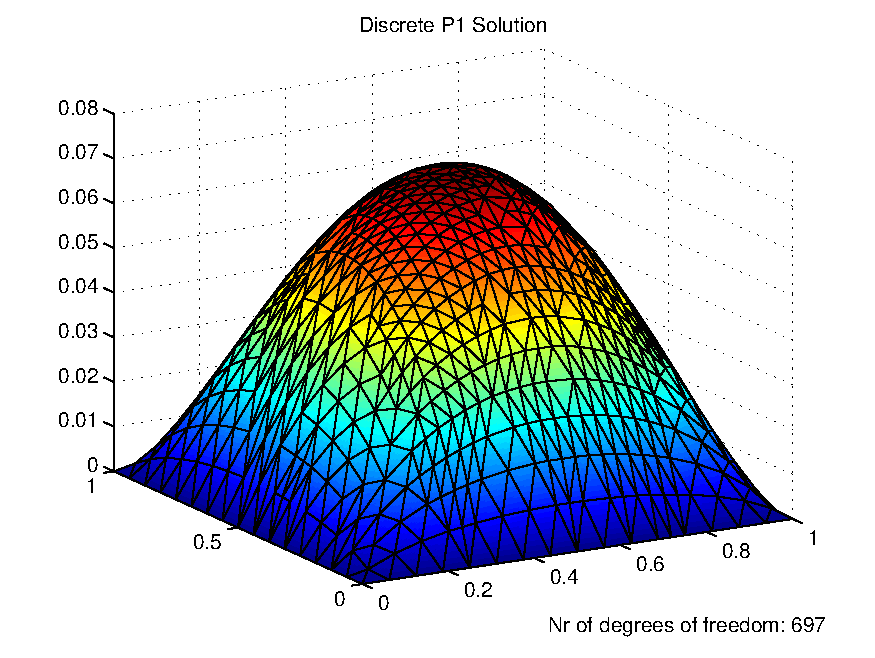
\includegraphics[width= 0.49\textwidth]{images/sect_QuickStart_Elliptic_Square_U}
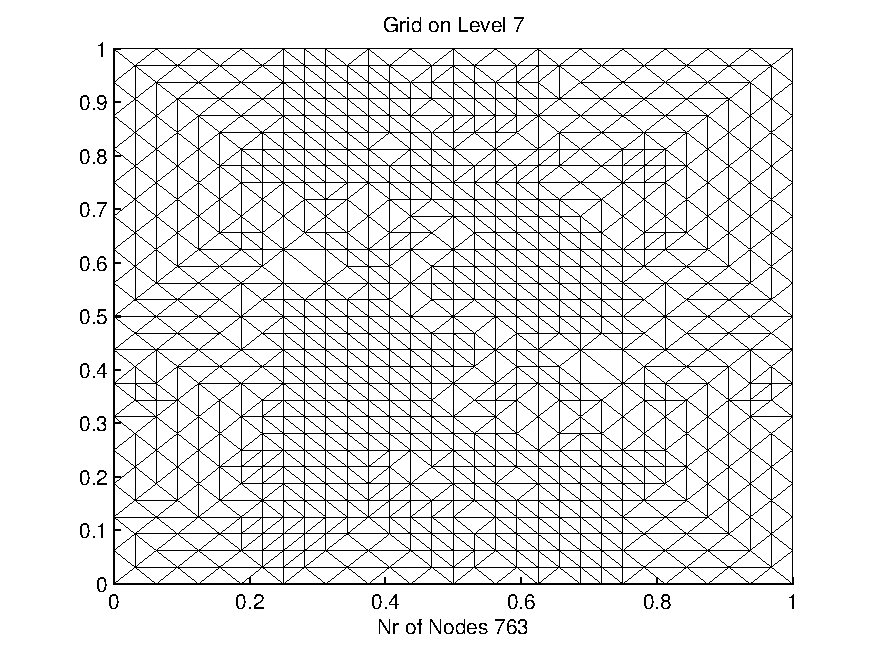
\includegraphics[width= 0.49\textwidth]{images/sect_QuickStart_Elliptic_Square_Mesh}
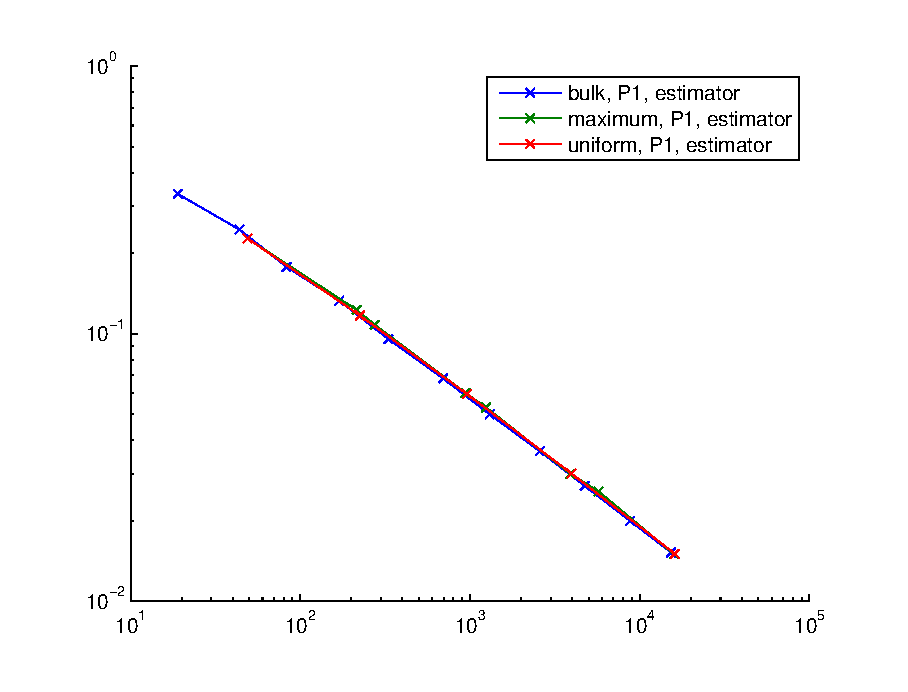
\includegraphics[width=0.8\textwidth]{images/sect_QuickStart_Elliptic_Square_Error}
\caption{ Plots for the example \code{Elliptic-Square}}
\label{sect:QuickStart:fig:Elliptic_Square}
\end{figure}

\clearpage

\subsubsection{$P_1$ FEM for the Elliptic-Lshape Problem}
\begin{align*}
-\Delta u &= 1 \textrm{ in } \Omega\\
 u &= 0 \textrm{ on } \partial\Omega
\end{align*}
In this example $\Omega$ is the L-shaped domain.
The solution is at least in $H^{5/3}(\Omega)$,
 therefore the expected convergence rate of the $H^1$ semi-error 
is $O(h^{2/3})$. Thus the convergence rate with respect to the 
degrees of freedom should be $N^{1/3}$ using uniform refined meshes,
see Figure~\ref{sect:QuickStart:fig:Elliptic_Lshape}.\bigskip

\begin{figure}[ht!]
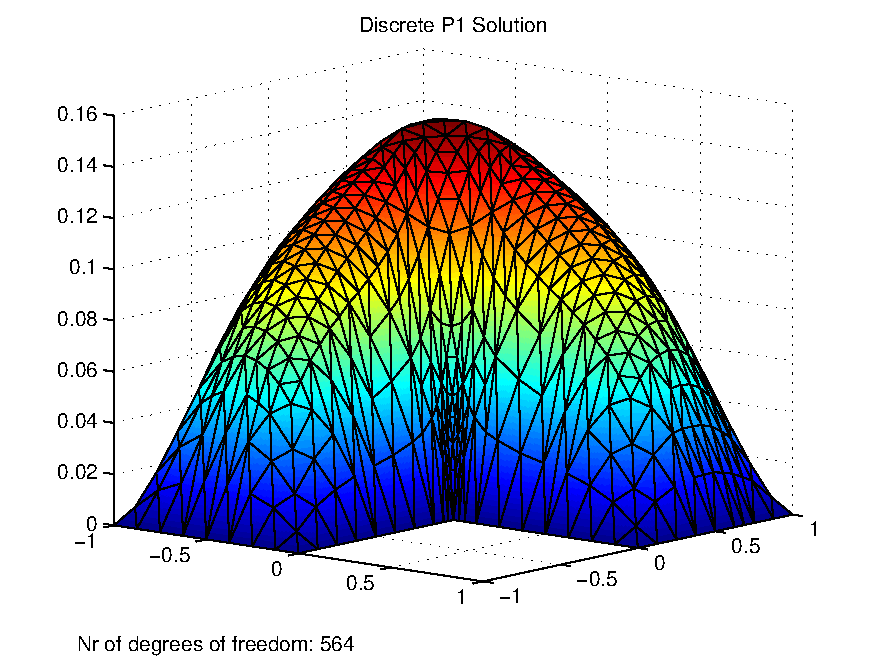
\includegraphics[width= 0.49\textwidth]{images/sect_QuickStart_Elliptic_Lshape_U}
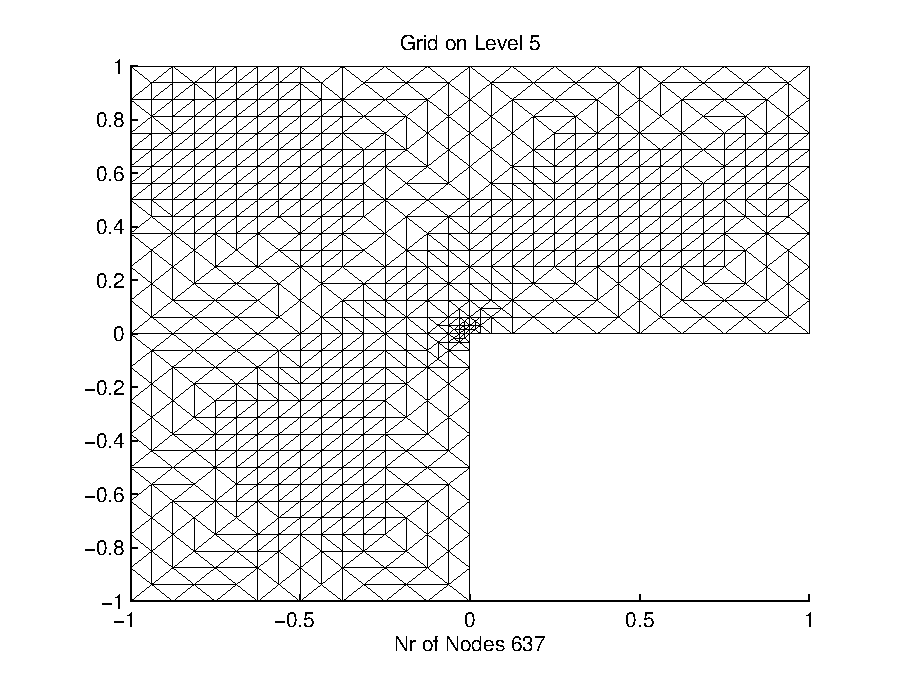
\includegraphics[width= 0.49\textwidth]{images/sect_QuickStart_Elliptic_Lshape_Mesh}\bigskip\\
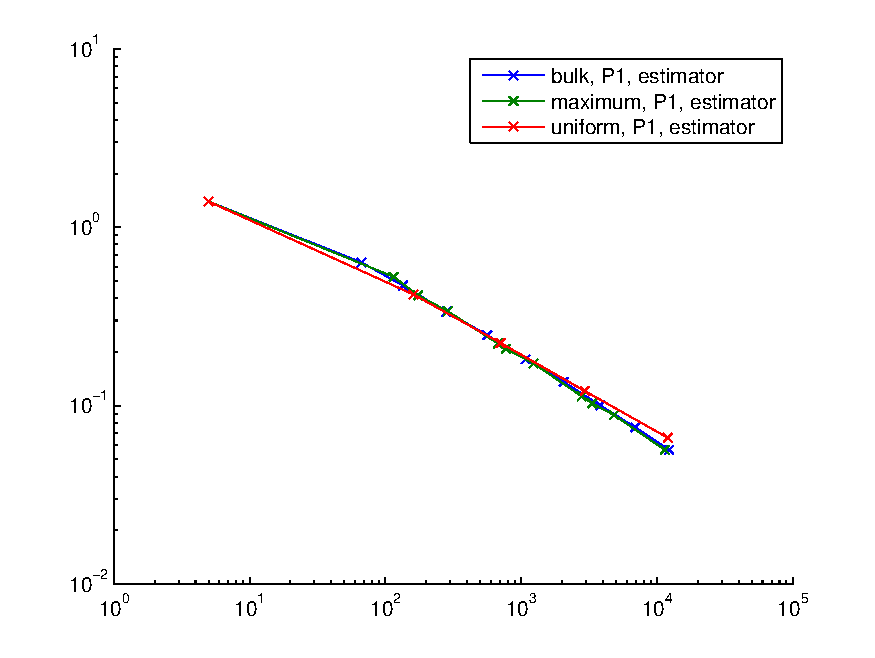
\includegraphics[width=0.9\textwidth]{images/sect_QuickStart_Elliptic_Lshape_Error}
\caption{ Plots for the example \code{Elliptic-Lshape}}
\label{sect:QuickStart:fig:Elliptic_Lshape}
\end{figure}

\clearpage

\subsubsection{$P_1$ FEM for the Elliptic-Square-exact Problem}
\begin{align*}
-\Delta u &= 2(x(1-x)+y(1-y)) \textrm{ in } \Omega\\
 u &= 0 \textrm{ on } \partial\Omega
\end{align*}
The exact solution for the unit square is given by $u=x(1-x)y(1-y)$. 
The Convergence rate is $O(h)$ for the energy error and because of Aubin-Nietsche $O(h^2)$ for the $L^2$-error, see Figure~\ref{sect:QuickStart:fig:Elliptic_Square_exact}.\bigskip

\begin{figure}[ht!]
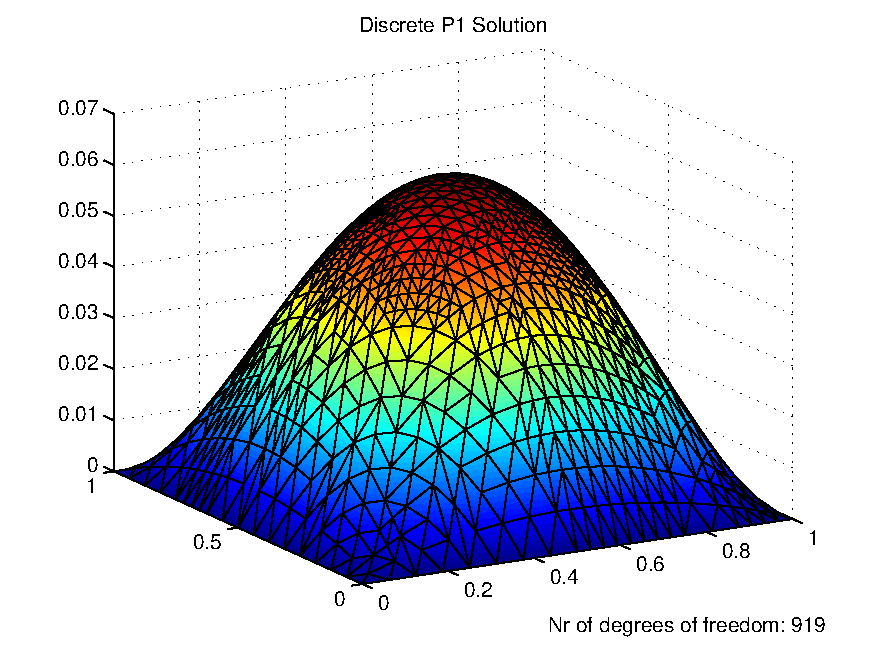
\includegraphics[width= 0.49\textwidth]{images/sect_QuickStart_Elliptic_Square_exact_U}
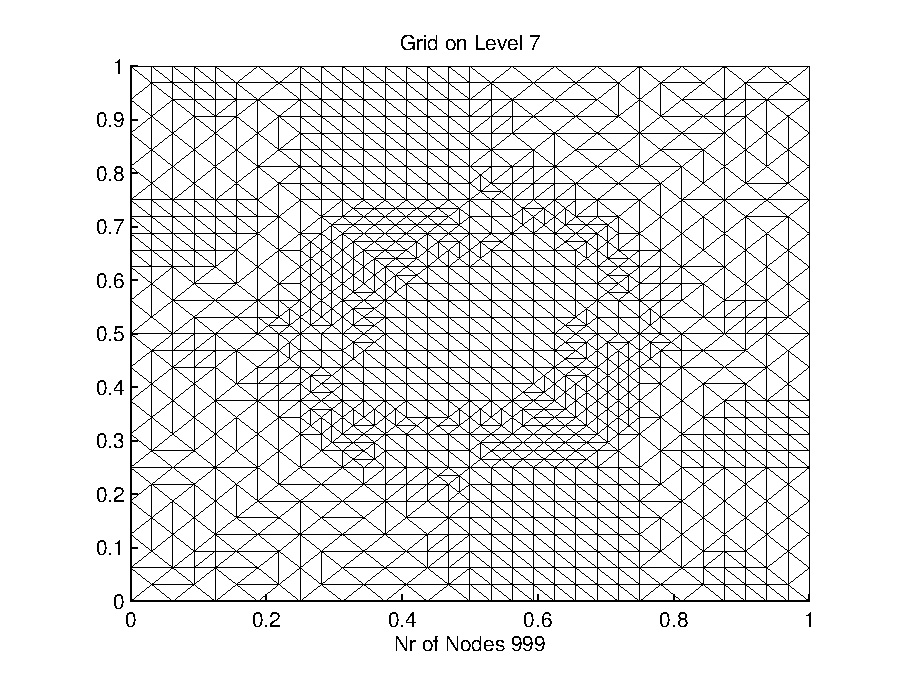
\includegraphics[width= 0.49\textwidth]{images/sect_QuickStart_Elliptic_Square_exact_Mesh}\bigskip\\
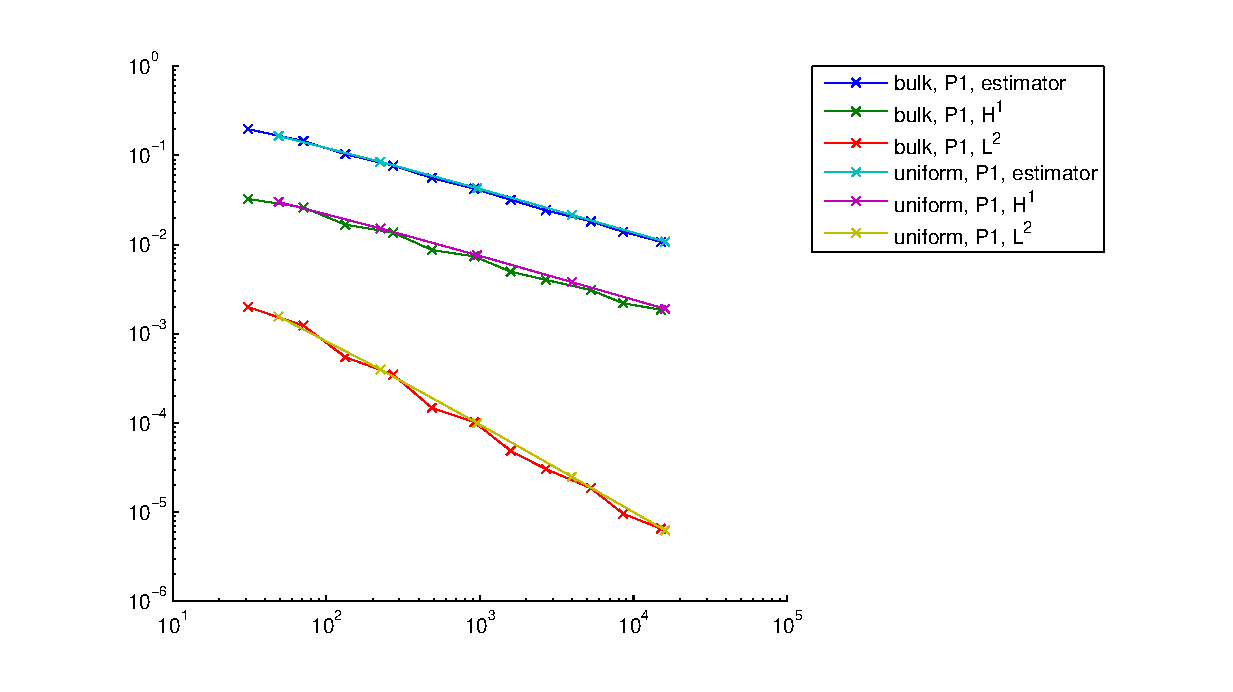
\includegraphics[width=0.9\textwidth]{images/sect_QuickStart_Elliptic_Square_exact_Error}
\caption{ Plots for the example \code{Elliptic-Square-exact}}
\label{sect:QuickStart:fig:Elliptic_Square_exact}
\end{figure}

\clearpage

\subsubsection{$P_1$ FEM for the Elliptic-Lshape-exact Problem}
\begin{align*}
-\Delta u &= 0 \textrm{ in } \Omega\\
 u &= 0 \textrm{ on } \Gamma_D =\{ (x=0 \wedge y\in[0,-1]) \vee (y=0 \wedge x\in[0,1])\}\\
 \partial u \cdot \nu &= g(x) \textrm{ on } \Gamma_N = \partial\Omega\backslash\Gamma_D
\end{align*}
The exact solution given in polar coordinates is $u=r^{2/3}\sin(2/3\phi)$ for  the L-shaped domain. 
Uniform meshes yield a convergence rate of $O(h^{2/3})$ for the energy error and $O(h^{4/3})$ for the $L^2$ error,
see Figure~\ref{sect:QuickStart:fig:Elliptic_Lshape_exact}.\bigskip

\begin{figure}[ht!]
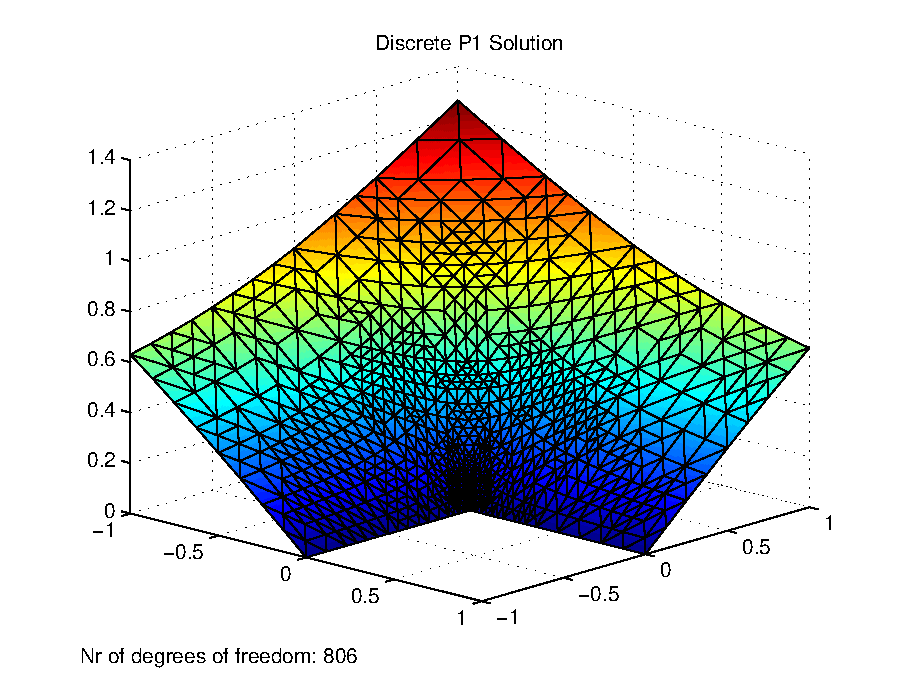
\includegraphics[width= 0.49\textwidth]{images/sect_QuickStart_Elliptic_Lshape_exact_U}
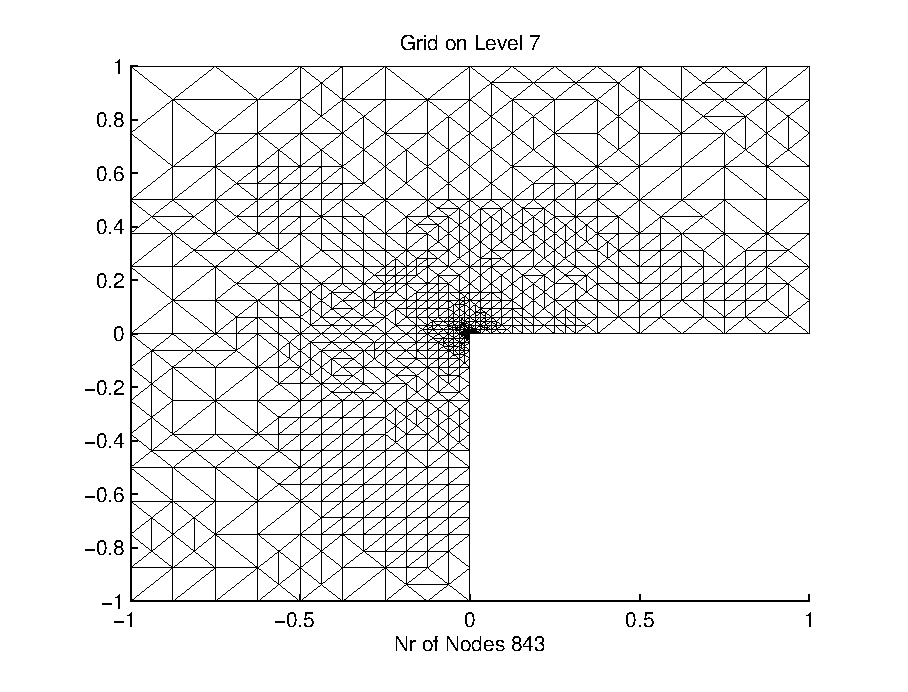
\includegraphics[width= 0.49\textwidth]{images/sect_QuickStart_Elliptic_Lshape_exact_Mesh}\bigskip\\
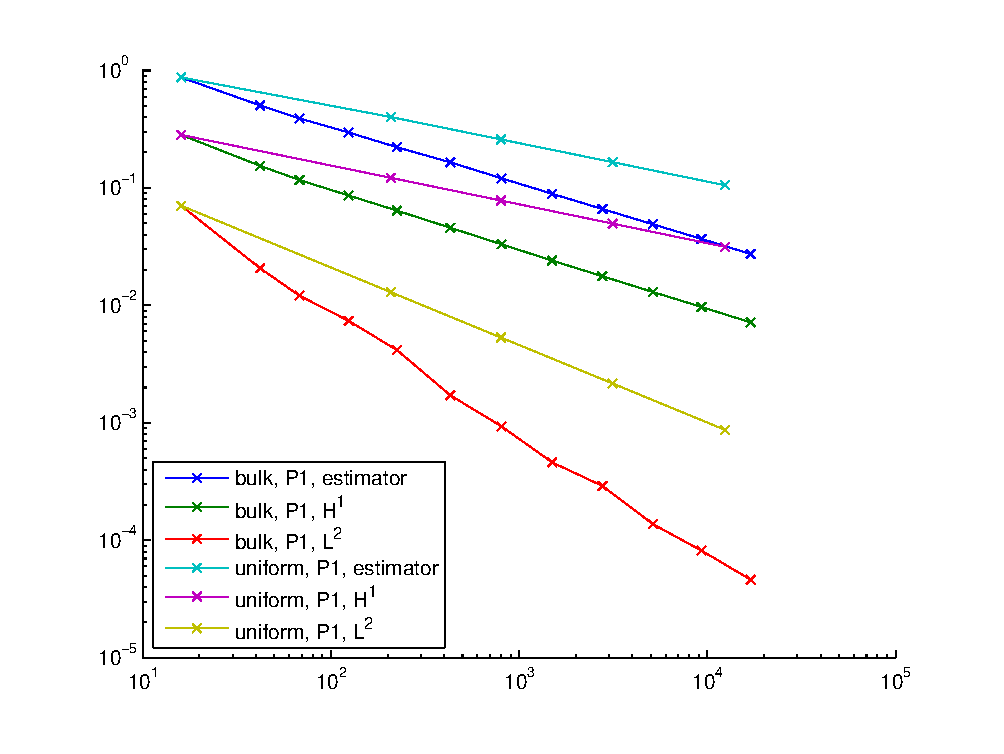
\includegraphics[width=0.9\textwidth]{images/sect_QuickStart_Elliptic_Lshape_exact_Error}
\caption{ Plots for the example \code{Elliptic-Lshape-exact}}
\label{sect:QuickStart:fig:Elliptic_Lshape_exact}
\end{figure}

\clearpage

\subsubsection{$P_1$ FEM for the Elliptic-Waterfall Problem}
\begin{align*}
-\Delta u &= f(x,y) \textrm{ in } \Omega\\
 u &= 0 \textrm{ on } \partial\Omega
\end{align*}
The exact solution is given by 
\[u = xy(1-x)(1-y)\textrm{atan}(k(\sqrt{(x-5/4)^2 + (y+1/4)^2}-1))\]
for the unit square. 
The convergence rate for the energy error is $O(h)$ 
whereas for the $L^2$-error it is $O(h^2)$. 
For $k\to\infty$ the slope of the function in special points tends to infinity, see Figure~\ref{sect:QuickStart:fig:Elliptic_Waterfall}.\bigskip

\begin{figure}[ht!]
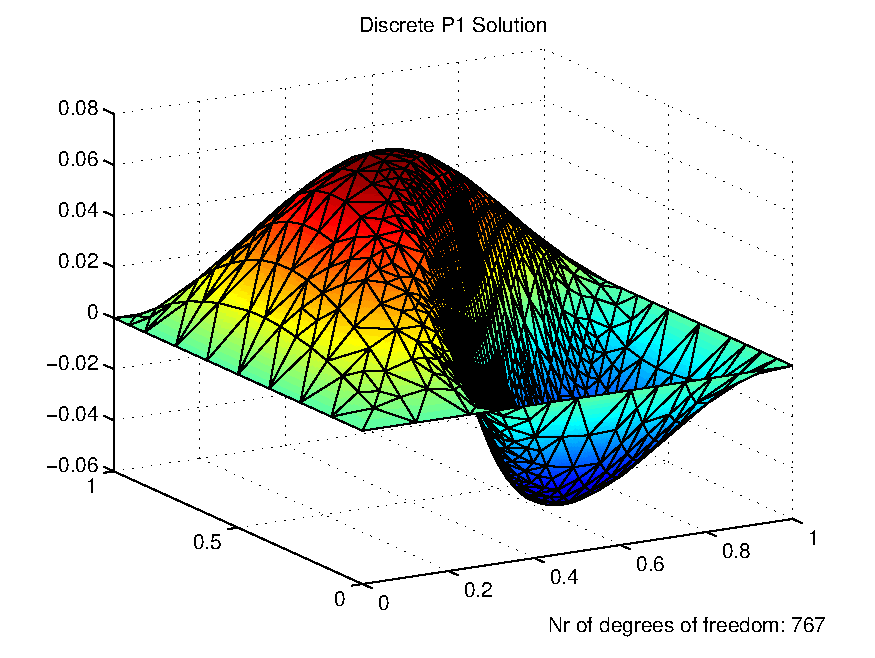
\includegraphics[width= 0.49\textwidth]{images/sect_QuickStart_Elliptic_Waterfall_U}
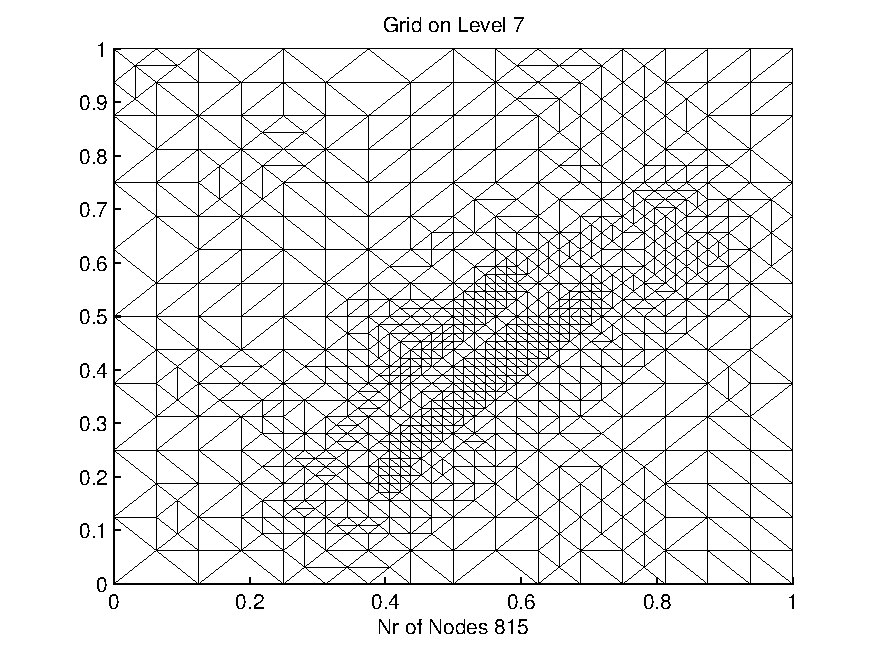
\includegraphics[width= 0.49\textwidth]{images/sect_QuickStart_Elliptic_Waterfall_Mesh}\bigskip\\
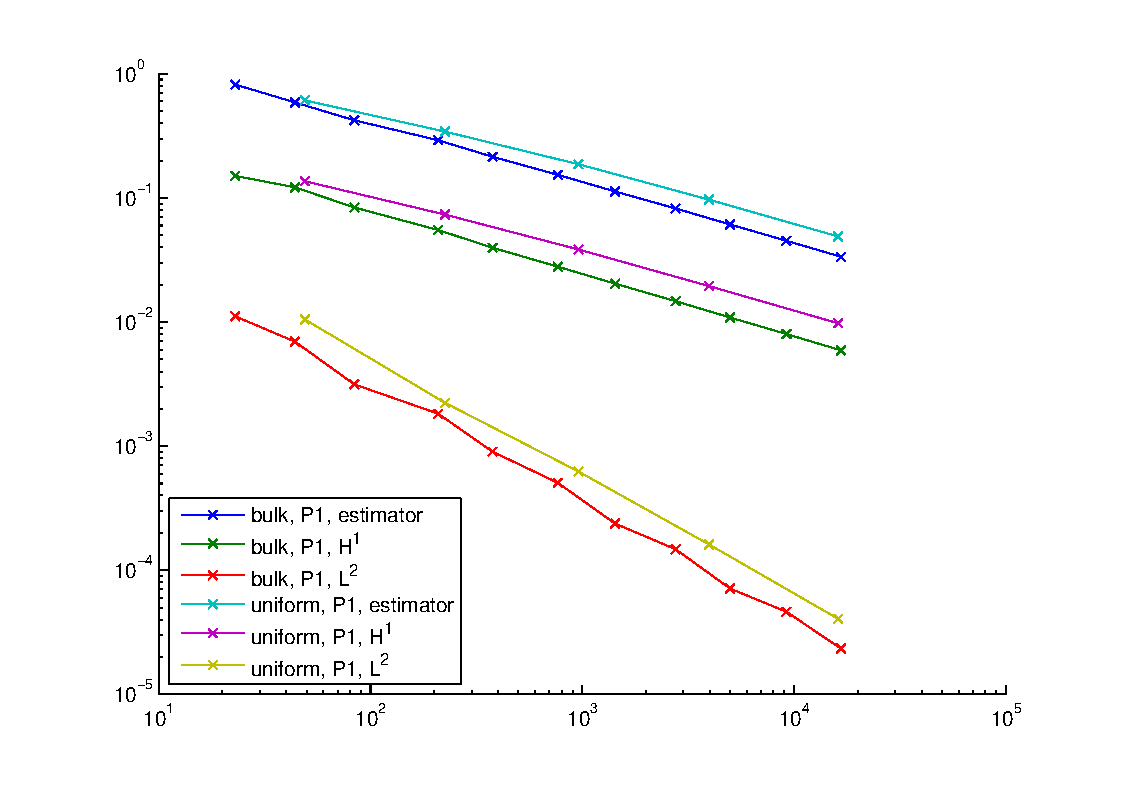
\includegraphics[width=0.9\textwidth]{images/sect_QuickStart_Elliptic_Waterfall_Error}
\caption{ Plots for the example \code{Elliptic-Waterfall}}
\label{sect:QuickStart:fig:Elliptic_Waterfall}
\end{figure}

\clearpage